\chapter{Mottos}\label{ch:mottos}

\begin{wrapfigure}{R}{0.3\textwidth}
    \centering
    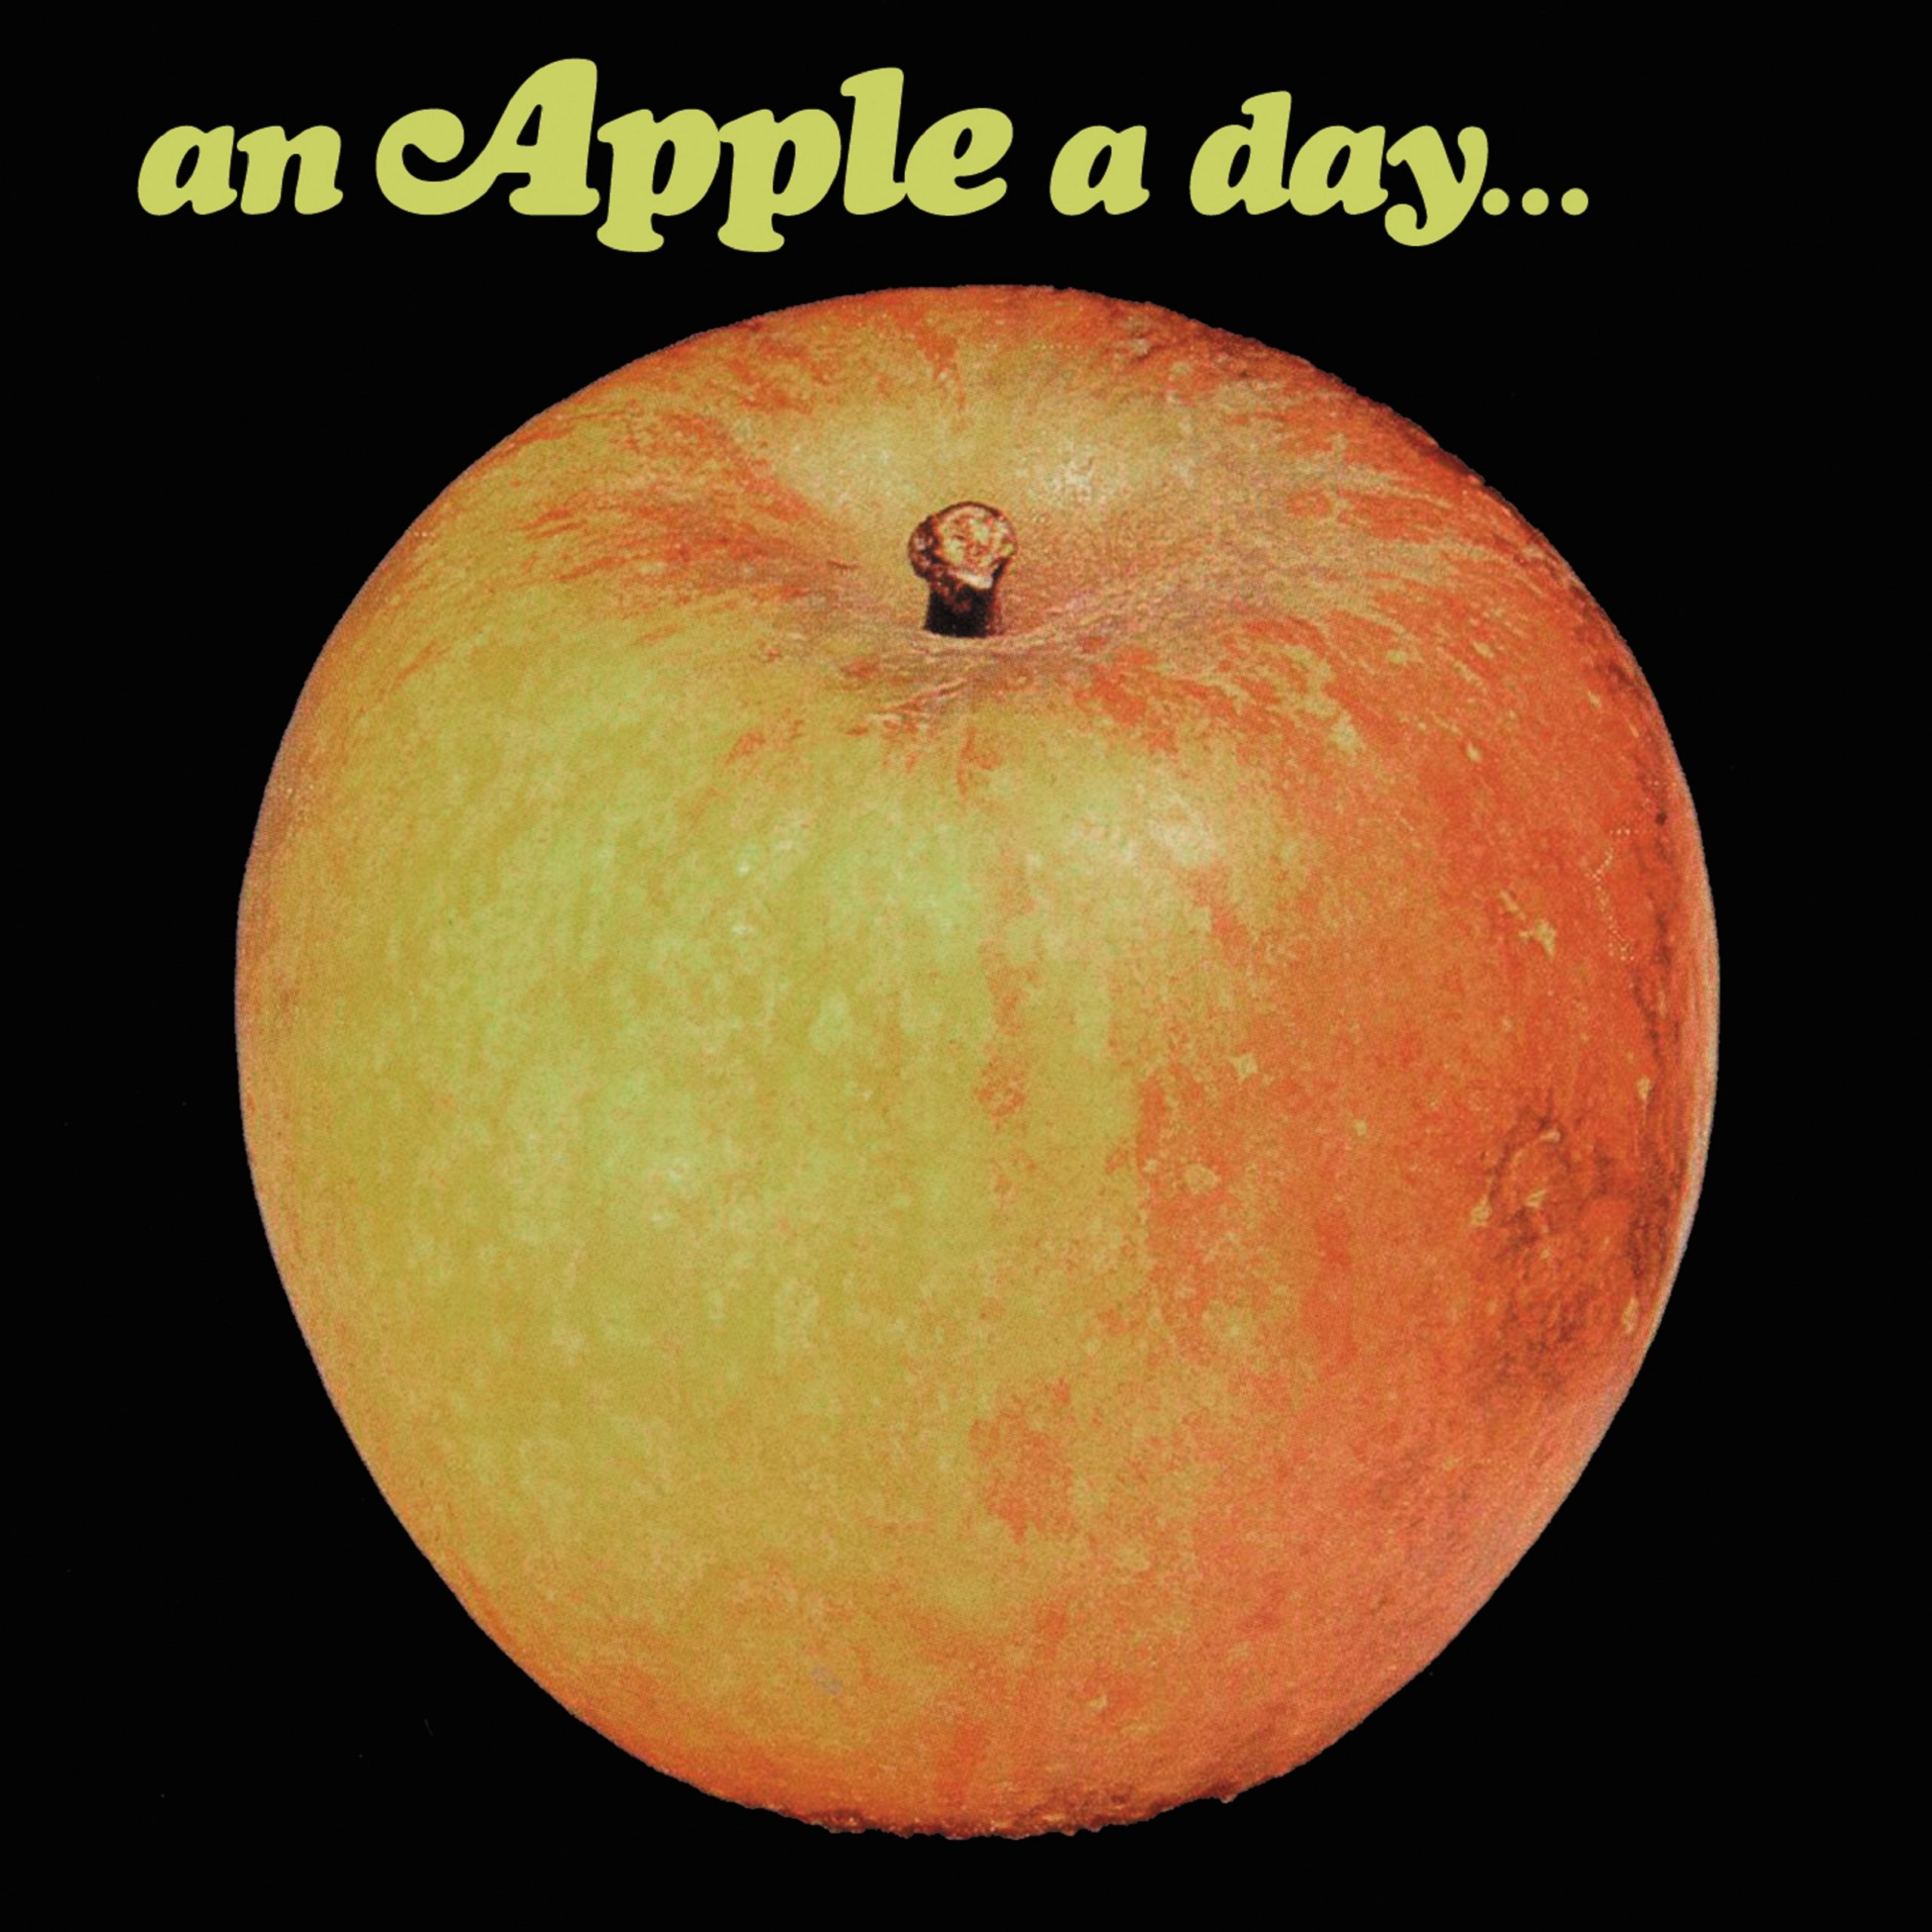
\includegraphics[width=0.25\textwidth]{images/mottos}
\end{wrapfigure}

You could also call them --universal-- guidelines, which would be semantically more specific than principles, yet not as specific as concrete techniques.
They help us improve our technique, implement the principles, and embody a quality more conforming to the core of CI\@.
They are kept short, so we can remember them quickly, and can act as part of our vocabulary.
Once we mention it to someone who is also familiar with that saying, we immediately have a common understanding within a very short period of time; something that is identical to the benefit of introducing a~\nameref{ch:jargon}.

\begin{itemize}
    \item [] \textit{Tension masks sensation.} \\
    Imagine your muscles are tensing up so much, they squeeze the nerves which then can't transmit any information anymore.
    The more \textbf{relaxed} we are, the more sensitive our skin is to touch, pressure and weight.
    Of course, we want to relax, yet not totally collapse, yet maintaining the minimum effort possible to stay stable; as little as possible, as much as necessary.
    \item [] \textit{Keep on breathing.} \\
    When getting tensed up, physically and/or emotionally, we tend to hold our breath, which is counterproductive to stay sharp, focused and relaxed.
    Instead, we continuously try to remind ourselves to breathe, and especially emphasize a deep out-breath, as the breathing out activates more our relaxation system; the parasympathetic nervous system to be precise.
    Whenever you realize that your partner becomes a bit stiff and holds his breath, it can be an effective way to non-verbally manipulate your partner into taking a big sigh as well, if you do it deliberately loud enough that he will hear it.
    It's a little bit like with the phenomena of yawning: Due to our social nature, equipped with mirror neurons, those behaviors tend to be contagious, and we can't help it but imitate it.
    \item [] \textit{We try not to fall in love with our partner, we fall in love with the dance.} \\
    Try to \textbf{depersonalize} your dance partner, seeing him as a mere physical object and by that explore the physical realm instead of the psychological, the interpersonal realm.
    It's also not a personal dance, it's a physicality; the experience is because of the practice, not because of your partner necessarily; don't attach that to a specific person, just like the teachings of Tantra tell us as well.
    Even when you had an amazing dance with someone, once the dance is over, I'm going to say ``Thank you, and bye bye''.
    It is nevertheless possible of course to talk to that person later on, but please don't linger and dance the entire class or jam with that single person.
    \item [] \textit{Keep eyes open and ``wide''.} \\
    Sometimes people tend to close their eyes, or focus them constantly, fierce-fully on the partner.
    Instead, we want to keep an open gaze, perceiving everything around us, staying in connection with all the people in the room and the room itself.
    Once we start to gaze at the floor, this is usually an indication of a state of hyper-focus, which potentially closes our perception.
    Remind yourself to keep your vision leveled, stay aware and attentive.
    \item [] \textit{Dance at the edge of your level of attention, and don't cross the level of your partner's attention.} \\
    Try to \textbf{expand} what you are able to do in regard to movement, attention, speed, techniques, and pathways.
    And very important, listen to what your partner is able as well, and \textbf{respect} that with patience and compassion.
\end{itemize}

\section{Inspirational Mistakes}\label{sec:inspirational-mistakes}

As in general with any improvised art, mistakes are only seen as such, as soon as we declare them as being mistakes.

\begin{displayquote}
    \textit{
Imagine two improvisation actors on stage.
One says ``mouse'', the other says ``house''.
And then again, the same thing: house, then mouse.
They actually intended to go on with different rhyming words, but for whatever reason (too nervous?) they are stuck and can't come up with something new, and because they are able to fake it as a deliberate decision (not admitting it being a mistake, something which was not their initial desired goal; when things don't go according to a fixed plan), people in the audience might be amazed by the ``post-modern acting skills'' and interpret something into it which is actually not there.
    }
\end{displayquote}

Once you are able to let go of any plan, and be truly in the \textbf{present moment} with whatever is happening; once you are able to fully comprehend that whenever there is another person involved, any desire for control is futile \ldots then you will be able to surrender and use any happening as a source of inspiration.
Ultimately being able to \textbf{surprise yourself}, and be fascinated what happened to you once you let go.
